\documentclass{beamer}

\usepackage{hyperref}
\usepackage{graphicx}

\title{Mobile Robot Systems Mini Project 5}
\author{Sam Sully (sjs252), Paul Durbaba (pd452), Luke Dunsmore (ldd25)}
\date{Lent 2020}
	
\begin{document}
		
	\frame{\titlepage}
		
	\begin{frame}
		\frametitle{Project Outline}
		\pause
		\begin{itemize}
			\item<2-> LIDAR based localisation (ex1)
			\item<3-> Improve with range and bearing of other robots (sjs252)
			\item<4-> Centralised approach to world coverage (ldd25)
			\item<5-> Decentralised approach to world coverage (pd452)
		\end{itemize}
	\end{frame}
	\begin{frame}
		\frametitle{Localisation}
		\pause
		\begin{itemize}
			\item<2->Particle filter
			\item<3->LIDAR
			\item<4->Range \& bearing
		\end{itemize}
	\end{frame}
	\begin{frame}
		\frametitle{LIDAR}
		\[
		w_i = \prod_{s_{j} \in \mathrm{Sensors}}\Phi(R(i,j), s_{ij}, \sigma^2)
		\]
		\begin{itemize}
			\item $w_i$ = LIDAR weight of particle $i$
			\item $s_{ij}$ = distance recorded by sensor $j$ on the robot
			\item $\Phi(x,\mu,\sigma)$ = Gaussian PDF with mean $\mu$ and standard deviation $\sigma$ 
			\item $R(i,j)$ = ray traced distance from particle $i$ in the direction of sensor $j$
		\end{itemize}
	\end{frame}
	\begin{frame}
		\frametitle{Range \& Bearing}
		\[
		\bar{w_i} = \prod_{r_j \in N_i}\sum_{p_k \in r_j}\Phi\left(
		\begin{bmatrix}
		D_i(p_k)\\
		\Theta_i(p_k)
		\end{bmatrix},
		\begin{bmatrix}
		d_j\\
		\theta_j
		\end{bmatrix},
		\xi
		\right) \cdot w_{p_k}
		\]
		\begin{itemize}
			\item $\bar{w_i}$ range \& bearing weight of particle $i$
			\item $N_i$ = robot $i$'s neighbours
			\item $p_k$ ranges over the set of particles from robot $r_j$ \item $d_j$ = received distance between this robot and robot $r_j$
			\item $\theta_j$ = received bearing of this robot from $r_j$
			\item $D_i(p_k)$  = distance between the particle $i$ on this robot and the particle $p_k$ from the other robot
			\item $\Theta_i(p_k)$ = bearing between the particle $i$ and the particle $p_k$ on the other robot
			\item $w_{p_k}$ = weight of particle $k$
			\item $\xi$ = covariance matrix
		\end{itemize}
		Normalising factors omitted.
	\end{frame}	
	\begin{frame}
		\frametitle{Performance Without Enhancement}
		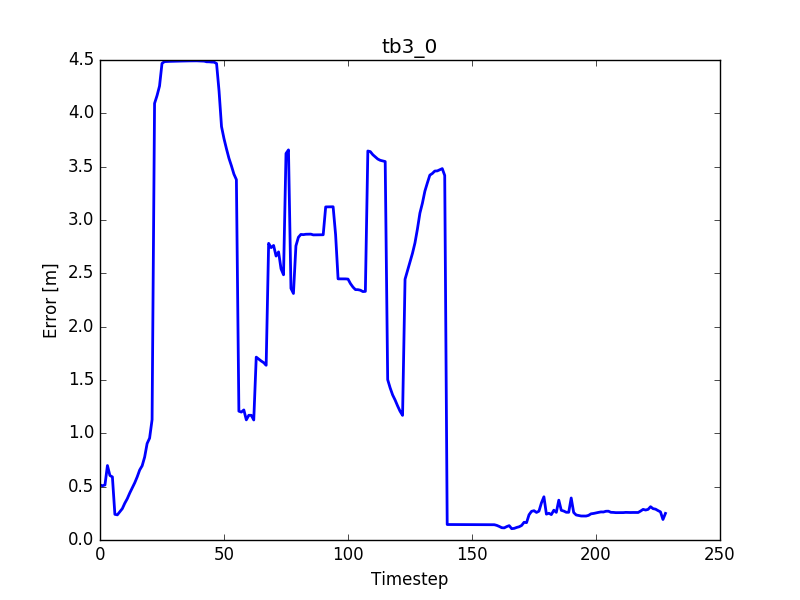
\includegraphics[width=\columnwidth]{figure_l2.png}
	\end{frame}
	\begin{frame}
		\frametitle{Performance With Enhancement}
		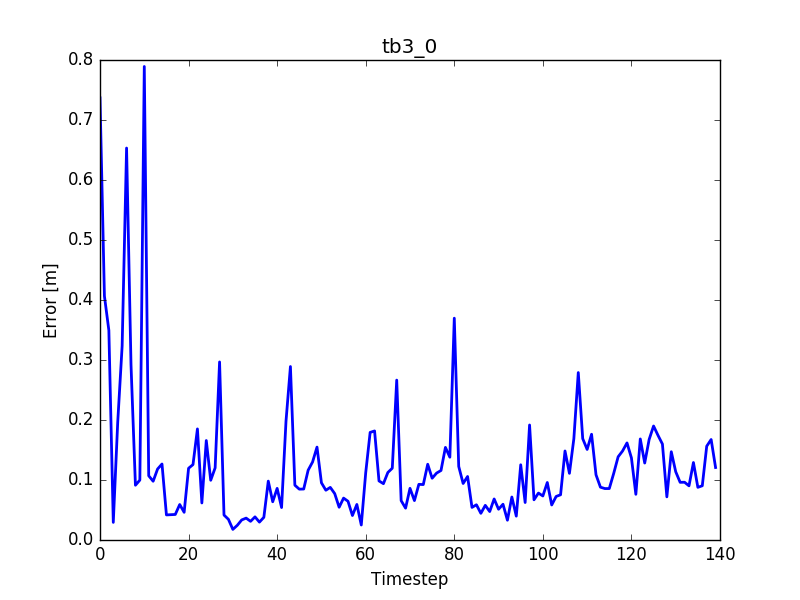
\includegraphics[width=\columnwidth]{figure_l1.png}
	\end{frame}
	\begin{frame}
		\frametitle{Demo}
		\url{https://drive.google.com/file/d/1VfTZwqM-bqTKb0AGtHgcXKm1kq8-nVVY/view?usp=sharing}
	\end{frame}
	
	%LUKE
	
	\begin{frame}
		\frametitle{Decentralized Coverage}
		\begin{itemize}
			\item Region Trading
			\item Navigation within region
		\end{itemize}
	\end{frame}
	
	\begin{frame}
		\frametitle{Region Trading}
		\begin{itemize}
			\item Each robot starts out believing that it `owns' the whole world
			\item When robots meet, they trade individual grid cells to try and balance the amount they both have
			\item Converges after about 10-20 random robot pairing trades.
		\end{itemize}
		
	\end{frame}
	
	\begin{frame}
		\frametitle{Region Trading}
		
		\begin{columns}
			\column{0.5\textwidth}
			After 3 trades - some area still multiply owned
			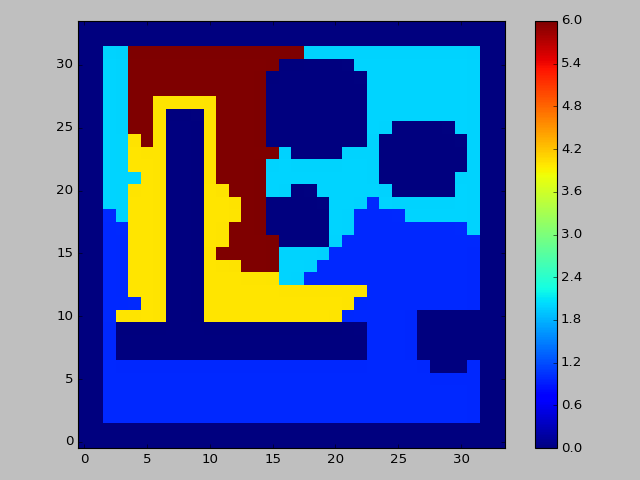
\includegraphics[width=\columnwidth]{rt_before.png}
			\column{0.5\textwidth}
			After 10 trades - regions are separate
			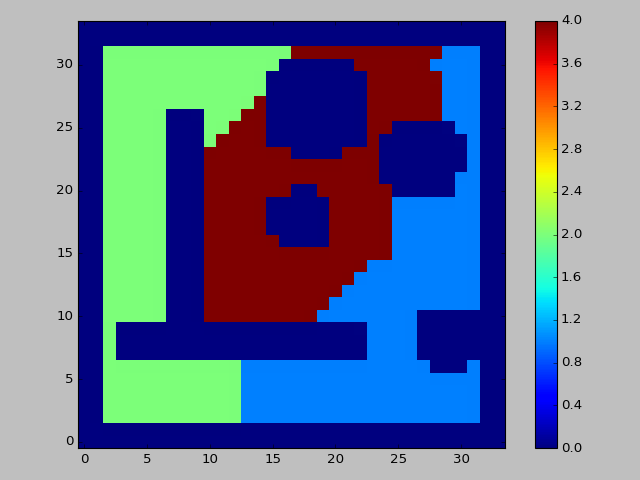
\includegraphics[width=\columnwidth]{rt_after.png}
		\end{columns}
	\end{frame}
	
	\begin{frame}
		\frametitle{Region Trading}
		\begin{itemize}
			\item Robots start by buying their positions
			\item Then take turns buying cells using BFS
			\item Cells already purchased by one robot can still be purchased by the other, if it has run out of unowned cells to buy
			\begin{itemize}
				\item Simple strategy used to avoid one robot accidentally splitting the other's region in two by doing this
			\end{itemize}
		\end{itemize}
	\end{frame}
	
	
	
	\begin{frame}
		\frametitle{Navigation within region}
		
		\begin{itemize}
			\item Two approaches tried
			\begin{itemize}
				\item Originally used RRT to each position - RRT leads to pathing everywhere
				\item Luke's strategy: Following around the MST of the region
			\end{itemize}
			\item The robots will always use RRT anyway to get back inside their region should they find themselves outside - hence paths outside of their own regions
		\end{itemize}
		
	\end{frame}
	
	\begin{frame}
		\frametitle{Collision avoidance}
		
		\begin{itemize}
			\item Phase 1 - modify speed / bearing to avoid potential collision
			\begin{itemize}
				\item Robots moving towards each other will bear away from each other
				\item Rotate away from line between the two robots
			\end{itemize}
			\item Phase 2 - cancel paths and switch to rule based movement away from obstacle / other robot
		\end{itemize}
	\end{frame}
	
	\begin{frame}
		\frametitle{Following MST}
		\begin{columns}
			\column{0.5\textwidth}
			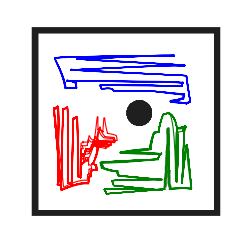
\includegraphics[width=\columnwidth]{dec2.png}
			\column{0.5\textwidth}
			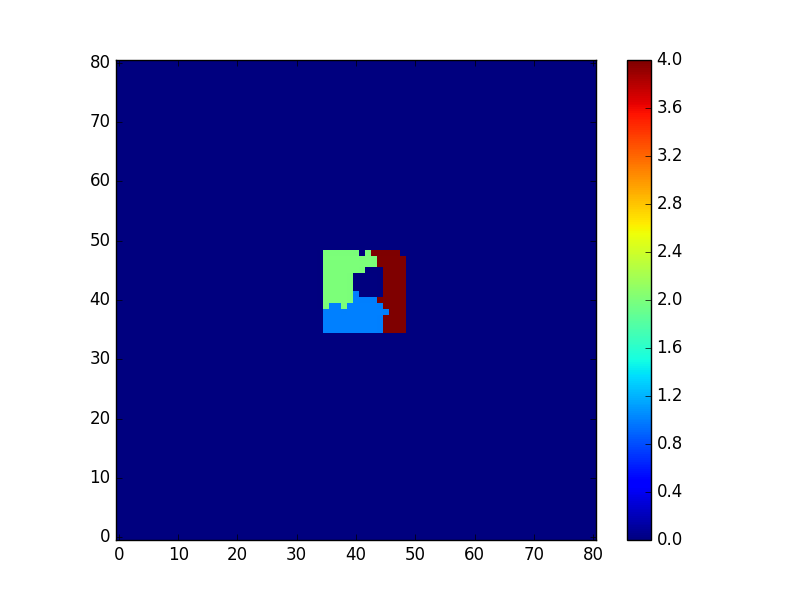
\includegraphics[width=\columnwidth]{owned_regions_2.png}
		\end{columns}
		
	\end{frame}
	
	\begin{frame}
		\frametitle{With Localization}
		\begin{columns}
			\column{0.5\textwidth}
			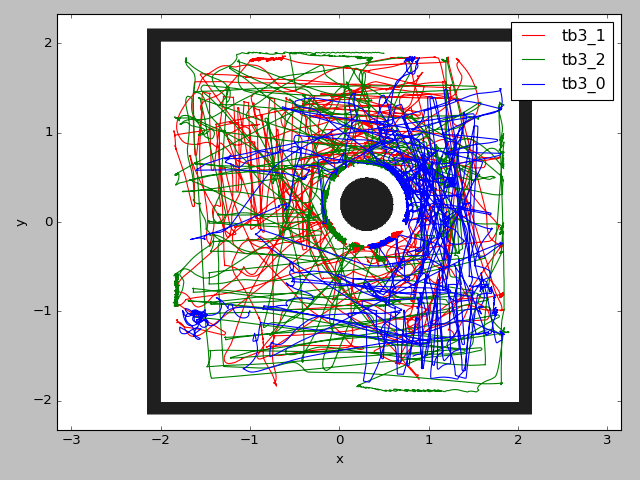
\includegraphics[width=\columnwidth]{dec_with_lo.png}
			\column{0.5\textwidth}
			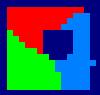
\includegraphics[width=\columnwidth]{or5.png}
		\end{columns}
	\end{frame}
\end{document}